\section{Theoretische Grundlage}
\label{sec:Theorie}
Es ist bekannt, dass Hüllenelektronen mit Bahndrehimpulsen ein magnetisches Moment besitzen. Allerdings zeigen Experimente, dass auch Elektronen mit einem verschwindendem Bahndrehimpuls ein magnetisches Moment besitzen. Dieses Phänomen wurde 1925 zum ersten mal entdeckt und wird Eigendrehimpuls oder Spin genannt. In diesem Versuch soll das magnetische Moment eines freien Elektrons und die Stärke des Erdmagnetfeldes bestimmt werden.



\subsection{Zusammenhang zwischen Bahndrehimpuls und magnetischem Moment}
Die Wellenfunktion $\Psi$ in der Einelektronennäherung eines Atoms ist gegeben als
\begin{align}
	\Psi_{n,l,m}(r,\theta,\phi) = R_{n,l}(r)\ \Theta_{l,m}\ \frac{\text{e}^{i\,m\,\psi}}{\sqrt{2\,\pi}} \ .
\end{align}
\hfill \footnotesize{($n$ = Hauptquantenzahl, $l$ = Bahndrehimpulsquantenzahl, $m$ = Orientierungsquantenzahl)} \hfill \vspace{0.25cm}\\
Die Stromdichte eines Teilchenstroms ist gegeben durch
\begin{align}
	S = \frac{\hbar}{2\,i\,m_0}\left( \Psi^*\,\nabla\,\Psi - \Psi\,\nabla\,\Psi^* \right) \ .
\end{align}
\hfill \footnotesize{($\hbar$ = reduziertes Plancksches Wirkungsquantum, $m_0$ = Ruhemasse eines Elektrons)} \hfill \vspace{0.25cm}\\
Da der Radialanteil $R$ und der Breitenkreisanteil $\Theta$ reelle Funktionen sind verschwinden $S_R$ und $S_\Theta$. Die azimutale Teilchenstromdichte ergibt sich zu
\begin{align}\label{eqn:aS} % azimutale Stromdichte
	S_\psi &= \frac{\hbar\,R^2\,\Theta^2}{2\,i\,m_0} \left( \frac{\text{e}^{-\,i\,m\,\psi}}{\sqrt{2\,\pi}} \frac{1}{r\,sin\,\theta} \frac{\partial}{\partial\,\psi} \frac{\text{e}^{i\,m\,\psi}}{\sqrt{2\,\pi}} - \frac{\text{e}^{i\,m\,\psi}}{\sqrt{2\,\pi}} \frac{1}{r\,sin\,\theta} \frac{\partial}{\partial\,\psi} \frac{\text{e}^{-\,i\,m\,\psi}}{\sqrt{2\,\pi}} \right) \nonumber \\
	&= \frac{\hbar\,R^2\,\Theta^2}{2\,\pi\,m_0}\frac{m}{r\,sin\,\theta}
\end{align}
Der durch das Flächenelement $df$ fließende Strom $dI_\psi$ beträgt
\begin{align}\label{eqn:Kreisstrom} % Kreisstrom
	dI_\psi = -\,e_0\cdot S_\psi\,df
\end{align}
\hfill \footnotesize{($e_0$ = Elementarladung)} \hfill \vspace{0.25cm}\\
Ein magnetisches Moment $d\mu_\text{z}$ entspricht dem Produkt aus dem Kreisstrom $dI_\psi$ und der umlaufenen Fläche $F(\theta) = \pi\, r^2\, sin^2\theta$. Mit den Gleichungen \eqref{eqn:aS} und \eqref{eqn:Kreisstrom} ergibt sich
\begin{align}\label{eqn:mM} % magnetisches Moment
	d\mu_\text{z} = F(\theta)\, dI_\psi = - \frac{e_0\, \hbar\, R^2\, \Theta^2}{2\, m_0} r^2\, sin\,\theta\, dr\, d\theta \ .
\end{align}
Durch Integration über die Elektronenhülle ergibt sich das gesamte magnetische Moment $\mu_\text{z}$ zu
\begin{align}\label{eqn:gmM} % gesamtes magnetisches Moment
	\mu_\text{z} = - \frac{e_0\, \hbar}{2\, m_0} m
\end{align}
Daraus folgt das Bohrsche Magneton $\mu_\text{B}$ \cite{V28}
\begin{align}\label{eqn:BM} % Bohrsches Magneton
	\mu_\text{B} = - \frac{e_0\, \hbar}{2\, m_0} = (\num{9.274015 +- 0.000003})\cdot 10^{-24} \frac{\text{J}}{\text{T}} \ .
\end{align}



\subsection{Drehimpulsquantelung und Energieniveauaufspaltung in einem Magnetfeld}

\begin{floatingfigure}{7cm}
	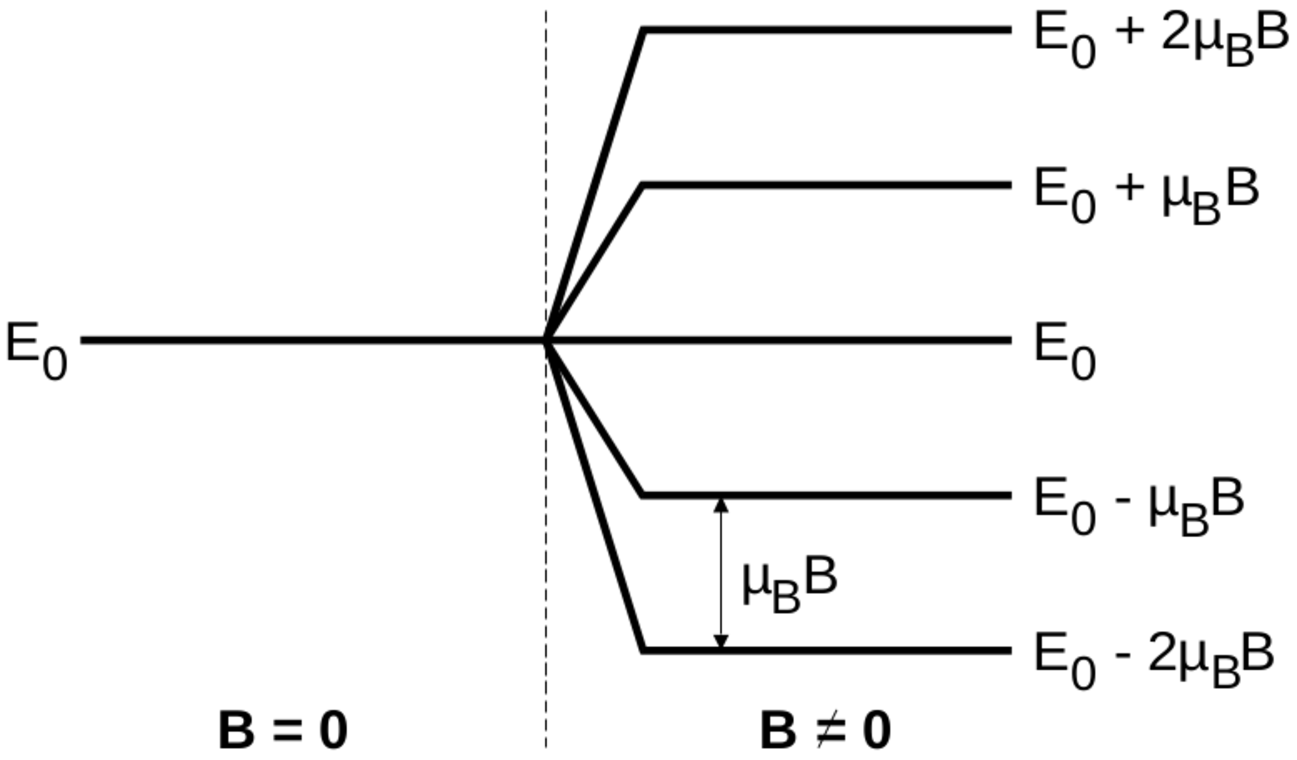
\includegraphics[width=7cm]{picture/Energiequantelung.pdf}
  \caption{Energieaufspaltung eines Hüllenelektrons in einem Magnetfeld mit $l = 2$. \cite{V28}}
	\label{fig:Energiequantelung}
\end{floatingfigure}

Neben der Quantelung des Drehimpulses, ist auch seine Richtung gequantelt. Die Drehimpulsrichtung $\vec{l}$ ist relativ zu einer Raumachse ausgerichtet, beispielsweise in Magnetfeldrichtung, sodass die $z$-Komponente $l_\text{z}$ nur ein ganzzahliges Vielfaches von $\hbar$ annehmen kann.
\begin{align}
	l_\text{z} = m_l\, \hbar
\end{align}
\hspace{1.9cm} \footnotesize{$(m_l = -l, \dots, 0, \dots, +l)$} \vspace{0.25cm}\\
Daher gibt es $2\,l + 1$ Einstellmöglichkeiten eines Drehimpulses bezüglich seiner Raumachse. Damit spaltet sich das Energiespektrum eines Elektrons im Magnetfeld in diskrete Energieniveaus auf
\begin{align}
	E_\text{mag} = m_l\, \mu_\text{B}\, B \ .
\end{align}
Diese Aufspaltung wird auch als Zeeman-Effekt bezeichnet. In Abbildung \eqref{fig:Energiequantelung} ist die Energieaufspaltung für $l = 2$ aufgezeigt. \\
Wird nun ein Elektronenstrahl durch ein in $z$-Richtung inhomogenes Magnetfeld geschickt, spaltet sich dieser in zwei Strahlen auf. Aus dieser Beobachtung folgt, dass Elektronen einen Spin mit zwei Ausrichtungsmöglichkeiten haben. Die Spinquantenzahl berechnet sich also mit
\begin{align*}
	&2\, s + 1 = 2 \\
	\Leftrightarrow &s = \frac{1}{2} \ .
\end{align*}
Daraus folgt für das magnetische Moment (siehe Gl. \eqref{eqn:gmM})
\begin{align*}
	\mu_{s_\text{z}} = -\,g \,m_s \,\mu_\text{B} = -\frac{\mu_\text{B}}{2}\, g
\end{align*}
\hfill \footnotesize{($g$ = Gyromagnetisches Verhältnis)} \hfill \vspace{0.25cm}\\
Ziel dieses Versuches ist es, dass Gyromagnetische Verhältnis zu bestimmen. Im Folgenden wird das, dafür verwendete, Messprinzip beschrieben.



\subsection{Messprinzip}
Das Gyromagnetische Verhältnis wird mit der Elektronenspin-Resonanz-Methode (kurz ESR) bestimmt. Dafür werden freie Elektronen in ein homogenes Magnetfeld gebracht, wodurch sich das Energieniveau in zwei Unterniveaus aufspaltet.

\begin{figure}[H]
	\centering
	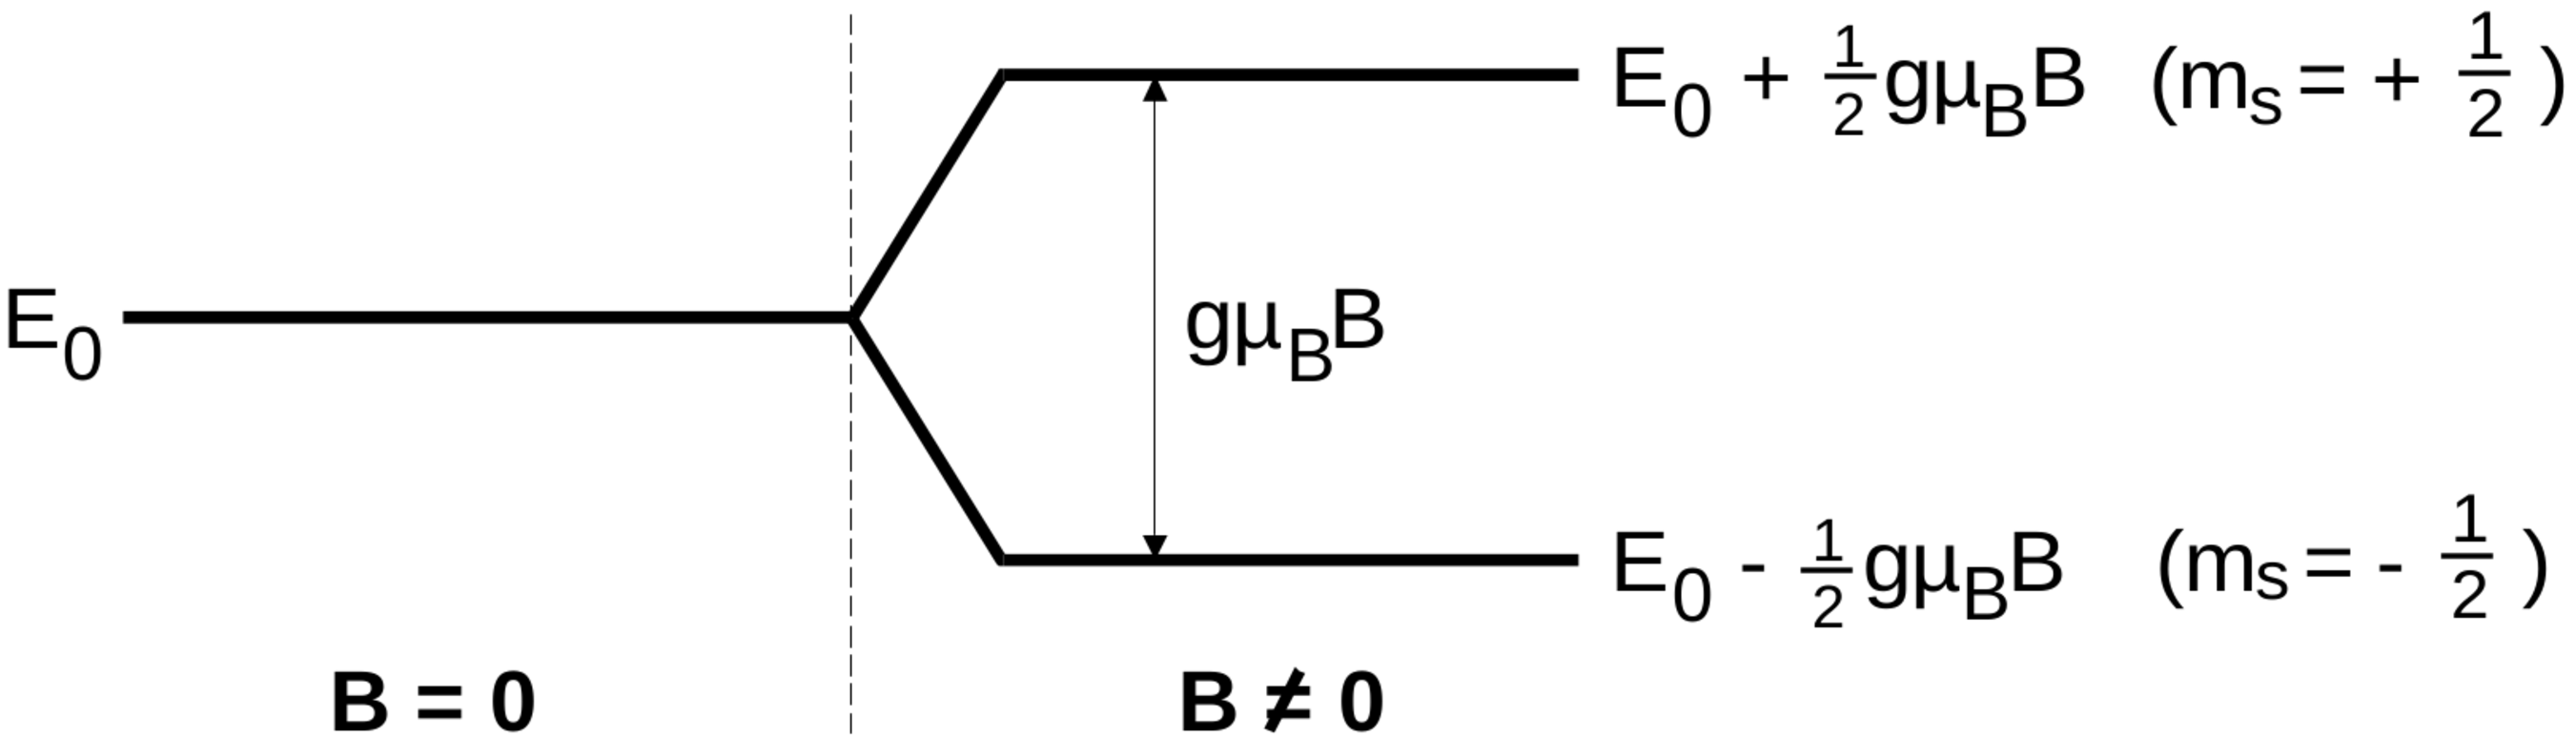
\includegraphics[width=\linewidth]{picture/EnergiequantelungElektron.pdf}
	\caption{Energieniveaus eines freien Elektrons in einem Magnetfeld. \cite{V28}}
	\label{fig:EnergiequantelungElektron}
\end{figure}

Nach der Maxwell-Boltzmann-Statistik ist der obere Zustand im thermischen Gleichgewicht weniger besetzt als der untere. Das Besetzungsverhöltnis ergibt sich zu
\begin{align}
	\frac{N(m_\text{s} = -\,\nicefrac{1}{2})}{N(m_\text{s} = \nicefrac{1}{2})} = \exp\left( \frac{-\,g\,\mu_\text{B}\,B}{k_\text{B}\,T} \right)
\end{align}
Die Elektronen können durch Photonen mit der richtigen Energie von dem Unteren Energieniveau in das höhere gehoben werden. Dazu muss die Energie der Photonen genau der Energiedifferenz zwischen den beiden Energieniveaus des Elektrons entsprechen.
\begin{align}
	h\,\nu = g\, \mu_\text{B}\, B
\end{align}
Dieser Vorgang wird als Elektronenspin-Resonanz bezeichnet.



\subsection{Magnetfeld einer Helmholtzspule}
Das Magnetfeld einer Helmholtzspule kann über
\begin{align}\label{eqn:BHelm} % B-Feld Helmholtzspule
	B = \frac{8}{\sqrt{125}}\, \frac{\mu_0\, n}{r}\, I
\end{align}
\hfill \footnotesize{($\mu_0$ = Induktionskonstnate, $n$ = Windungszahl, $r$ = Spulenradius, $I$ = Feldstrom)} \hfill \vspace{0.25cm}\\
berechnet werden.


\newpage
\subsection{Fehlerrechnung}
Sämtliche Fehlerrechnungen werden mit Hilfe von Python 3.4.3 durchgeführt.
\subsubsection{Mittelwert}
Der Mittelwert einer Messreihe $x_\text{1}, ... ,x_\text{n}$ lässt sich durch die Formel
\begin{equation}
	\overline{x} = \frac{1}{N} \sum_{\text{k}=1}^\text{N} x_k
	\label{eqn:ave}
\end{equation}
berechnen. Die Standardabweichung des Mittelwertes beträgt
\begin{equation}
	\Delta \overline{x} = \sqrt{ \frac{1}{N(N-1)} \sum_{\text{k}=1}^\text{N} (x_\text{k} - \overline{x})^2}
	\label{eqn:std}
\end{equation}

\subsubsection{Gauß'sche Fehlerfortpflanzung}
Wenn $x_\text{1}, ..., x_\text{n}$ fehlerbehaftete Messgrößen im weiteren Verlauf benutzt werden, wird der neue Fehler $\Delta f$ mit Hilfe der Gaußschen Fehlerfortpflanzung angegeben.
\begin{equation}
	\Delta f = \sqrt{\sum_{\text{k}=1}^\text{N} \left( \frac{ \partial f}{\partial x_\text{k}} \right) ^2 \cdot (\Delta x_\text{k})^2}
	\label{eqn:var}
\end{equation}

\subsubsection{Lineare Regression}
Die Steigung und y-Achsenabschnitt einer Ausgleichsgeraden werden gegebenfalls mittels Linearen Regression berechnet.
\begin{equation}
	y = m \cdot x + b
	\label{eqn:reg}
\end{equation}
\begin{equation}
	m = \frac{ \overline{xy} - \overline{x} \overline{y} } {\overline{x^2} - \overline{x}^2}
	\label{eqn:reg_m}
\end{equation}
\begin{equation}
	b = \frac{ \overline{x^2}\overline{y} - \overline{x} \, \overline{xy}} { \overline{x^2} - \overline{x}^2}
	\label{eqn:reg_b}
\end{equation}
